\documentclass{report}[11pt]
\usepackage[top=1.0in, bottom=1.0in, left=1.0in, right=1.0in]{geometry}
\usepackage{graphicx}
\usepackage{listings}
\usepackage{color}
\usepackage{setspace}
\usepackage{tocloft}
\doublespacing
\definecolor{dkgreen}{rgb}{0,0.6,0}
\definecolor{gray}{rgb}{0.5,0.5,0.5}
\definecolor{purple}{rgb}{0.73,0.33,0.83}
\lstset{language=Matlab,
   keywords={break,case,catch,continue,else,elseif,end,for,function,
      global,if,otherwise,persistent,return,switch,try,while,ones,
      squeeze,warning,waitbar,circshift},
   basicstyle=\ttfamily,
   keywordstyle=\color{blue},
   commentstyle=\color{dkgreen},
   stringstyle=\color{purple},
   numbers=left,
   numberstyle=\tiny\color{gray},
   stepnumber=1,
   numbersep=10pt,
   backgroundcolor=\color{white},
   tabsize=4,
   showspaces=false,
   showstringspaces=false,
   breaklines=true}
\renewcommand{\cftchapdotsep}{\cftdotsep}

\newenvironment{code}
{\begin{list}{}{\setlength{\leftmargin}{1em}}\item\scriptsize\bfseries}
{\end{list}}


\begin{document}
\newcommand{\signhere}{\vspace{0.4in}\rule{\linewidth}{0.5mm}\\}
% Everything is kept in seperate files.  Use this file to change the orders.
\pagenumbering{roman}
\thispagestyle{empty}
\begin{titlepage}
\begin{center}
\vspace*{\fill}
{ \huge \thesisTitle } \\
\vspace{1.0in}
by \\
\vspace{1.0in}
{ \large \textsc{Greggory H. Rothmeier} } \\
\vspace{2.0in}
A Thesis Submitted in Partial Fulfillment of the Requirements for the Degree of\\
Masters of Science\\
in the College of Arts and Sciences\\
Georgia State University\\
2012\\
\vspace*{\fill}
\end{center}
\end{titlepage}
Copyright
\thispagestyle{empty}
\begin{center}
  \textsc{\thesisTitle} \\
  \vspace{0.5in}
  by \\
  \vspace{0.5in}
  \textsc{Greggory H. Rothmeier} \\
  \vspace{1in}
\end{center}
\begin{flushright}
  \begin{doublespace}
    Committee Chair:~~~~A. G. Unil Perera \\
    Committee:~~~~Mukesh Dhamala \\
                 Brian Thoms \\
                 D. Michael Crenshaw \\
  \end{doublespace}
\end{flushright}
\vspace{0.5in}
\begin{flushleft}
  Electronic Version Approved: \\
  \vspace{0.5in}
  \begin{doublespace}
    Office of Graduate Studies\\
    College of Arts and Sciences\\
    Georgia State University\\
    May 2012\\
  \end{doublespace}
\end{flushleft}
\vspace*{\fill}
\phantomsection
\addcontentsline{toc}{chapter}{Dedication}
\begin{doublespace}
  \begin{center}
    \textbf{Dedication}
  \end{center}
This is dedicated to my parents who made me go to college and to Brooke who inspired me to go to graduate school.  If I wasn't lucky enough to have all of you I would probably be working for Geek Squad.
  
I also want to more specifically dedicate this to my mama.  I miss you and I think about you every day.
\end{doublespace}
\addcontentsline{toc}{chapter}{Acknowledgments}
\begin{doublespace}
  \begin{center}
    \textbf{Acknowledgements}
  \end{center}
  Perera, Dhamala, Brooke, Lab Mates, Dhamala's Lab
\end{doublespace}
\tableofcontents
\clearpage
\addcontentsline{toc}{chapter}{List of Tables}
\listoftables
\clearpage
\addcontentsline{toc}{chapter}{List of Figures}
\listoffigures
\begin{doublespace}
\begin{center}
  \textsc{Awesome title}\\
  \vspace{0.4in}
  A thesis\\
  presented in Partial Fulfilment of Requirements for the Degree of Master of Science in the\\
  College of Arts and Sciences\\
  Georgia State University\\
  2012\\
  by\\
  Greggory Rothmeier\\
  \vspace*{\fill}
  Committee:\\
  \begin{singlespace}
    \signhere
    A. G. Unil Perera, Chair\\
    \signhere
    Mukesh Dhamala, Member\\
    \signhere
    Brian Thoms, Member\\
    \signhere
    D. Michael Crenshaw, Member \\
    \vspace{0.2in}
    April 1, 2012\\
    \rule{\linewidth}{0.5mm}
    Date\\
    \signhere
    Dick Miller\\
    Department Chair\\
    \vspace{0.1in}
  \end{singlespace}
\end{center}
\end{doublespace}
\pagenumbering{arabic}
\setcounter{page}{1}
% List of Chapters in the order they need to appear
\chapter{Introduction}

% Why do temperature modeling?
% What level of temperature resolution is needed?
% What temperature resolution is available?
% How can we improve current detectors? (SP)


Since its invention in the 1950's~\citep{carr1954} and later development in the 1970's~\citep{lauterbur1973}, {M}agnetic {R}esonance {I}maging ({MRI}) has allowed physicians and scientists a detailed view within the human body.
  
  % MODELING BOLD
  \section{Models of the fMRI BOLD Response}
  \label{sec:BOLDmodeling}
  
  \begin{figure}[bt]
    \centering
    \vspace{10pt}
    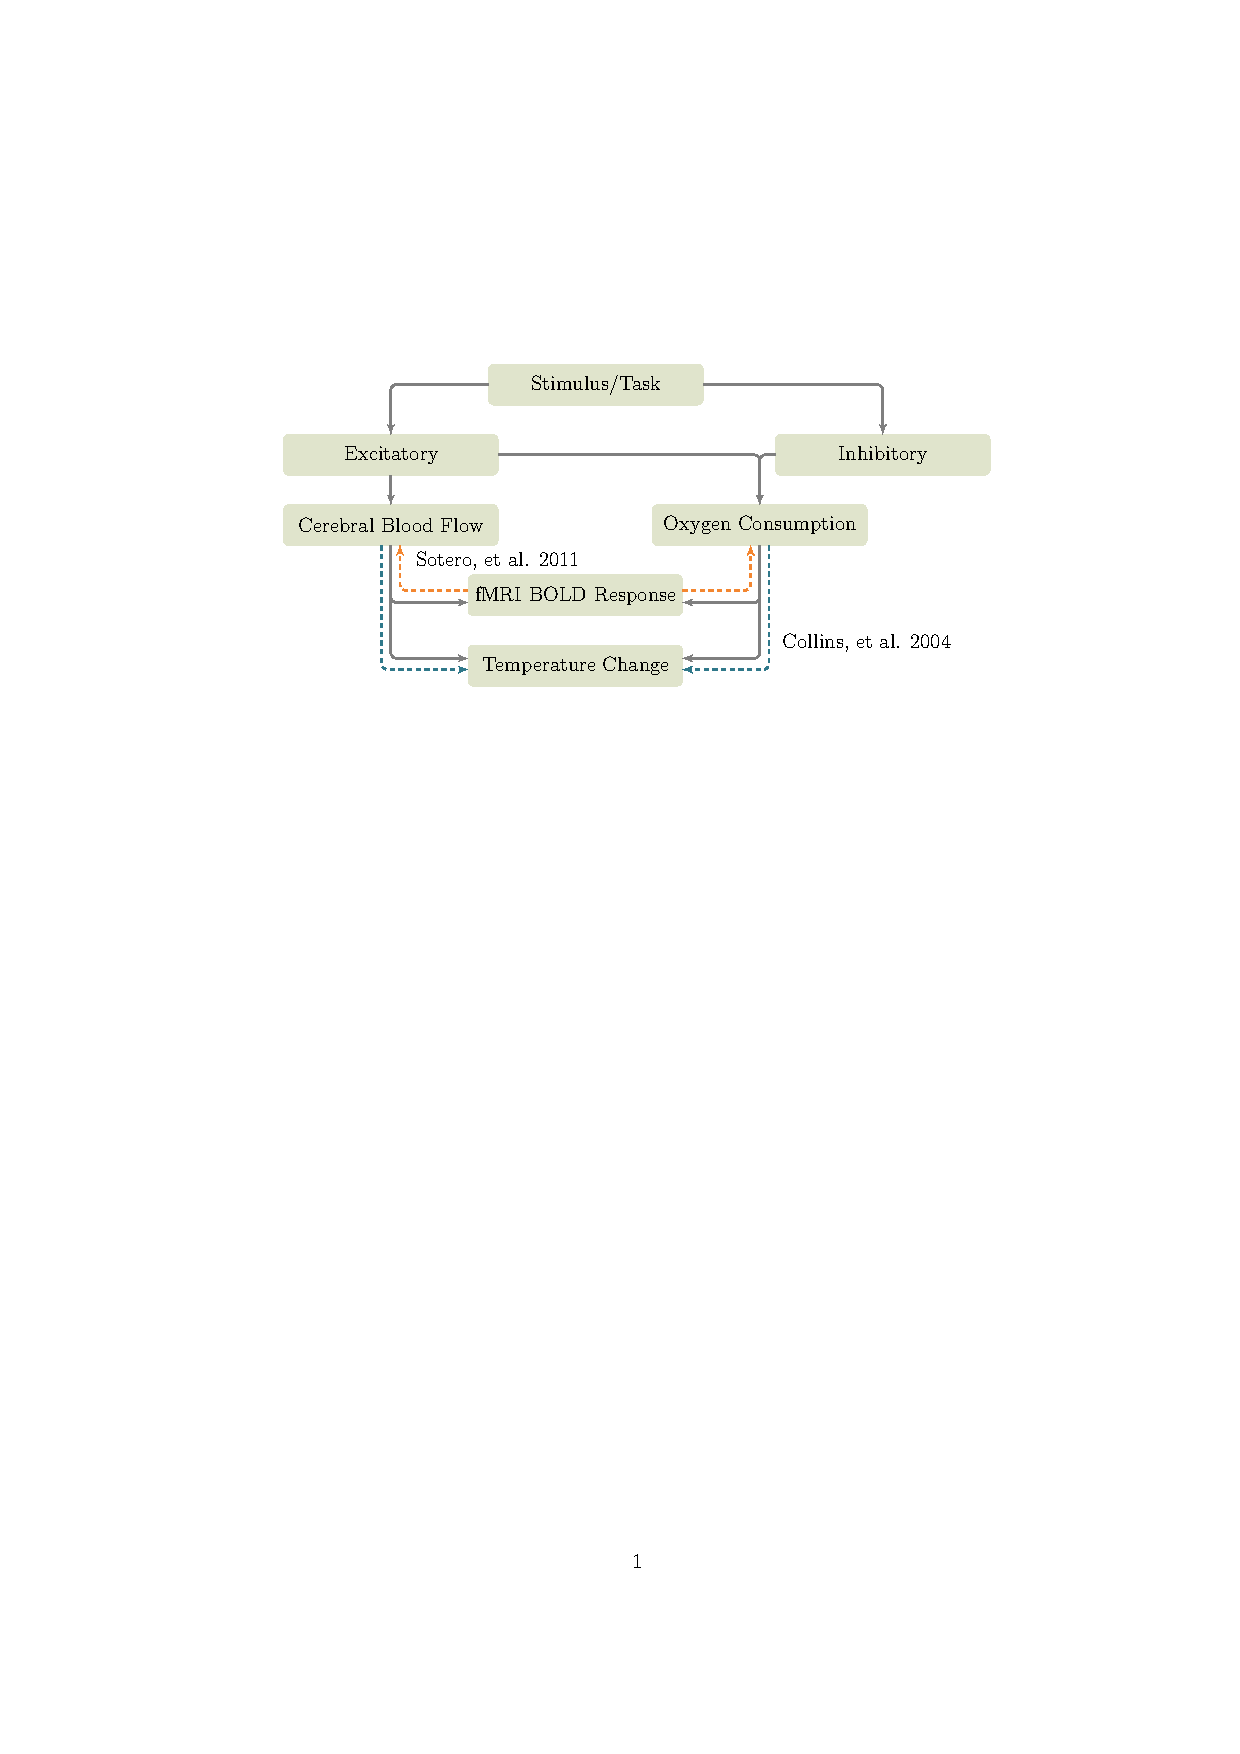
\includegraphics{flowchart}
    % \tikzstyle{block} = [draw=none, fill=beachstorm]
\tikzstyle{line} = [draw, very thick, color=black!50, -stealth']
\tikzstyle{sotero} = [draw, very thick, dashed, color=goldfish, -stealth']
\tikzstyle{collins} = [draw, very thick, dashed, color=aoi, -stealth']
\tikzstyle{citation} = [draw=none, fill=white, minimum height=0.5cm, anchor=north, text width=6.5cm]

\begin{tikzpicture}[node distance=0.7cm, rectangle, text width=4.5cm, text badly centered, rounded corners, minimum height=1cm, anchor=north]
  \node[block](stimulus){Stimulus/Task};
  
  \node[block, below=of stimulus, xshift=-5cm](excitatory){Excitatory Neuronal Activity};
  \node[block, below=of stimulus, xshift= 7cm](inhibitory){Inhibitory Neuronal Activity};
  
  \node[block, below=of excitatory](cbf){Increase in Cerebral Blood Flow (CBF)};
  \node[block, below=of inhibitory, xshift=-3cm](o2){Change in Oxygen Consumption (CMRO$_2$)};
  
  \node[block, below=of cbf, xshift=4.5cm, yshift=-0.5cm](bold){fMRI BOLD Response};
  \node[block, below=of bold](temp){Temperature Change};
  
  \node[citation](sotero1) at (-1.6, -5) {\citet{sotero2011}};
  % \node[citation](sotero1) at (2, -4.5) {Sotero, et. al. 2011};
  % \node[citation](sotero1) at (-4.5, -7.5) {Collins, et. al. 2011};
  \node[citation](sotero1) at (6, -6.5) {\citet{collins}};
  
  \path[line](stimulus.west) -| (excitatory.north);
  \path[line](stimulus.east) -| (inhibitory.north);
  \path[line](excitatory.south) -- (cbf.north);
  \path[line](excitatory.east) -| (o2.north);
  \path[line](inhibitory.west) -| (o2.north);
  
  \path[line](cbf.south) |- ([yshift=-5pt] bold.west);
  \path[line](cbf.south) |- ([yshift= 5pt] temp.west);
  \path[line](o2.south)  |- ([yshift=-5pt] bold.east);
  \path[line](o2.south)  |- ([yshift= 5pt] temp.east);
  
  \path[sotero]([yshift= 5pt] bold) -| ([xshift= 20pt] cbf);
  \path[sotero]([yshift= 5pt] bold) -| ([xshift=-20pt] o2);
  \path[collins]([xshift=-45pt] cbf) |- ([yshift=-5pt] temp);
  \path[collins]([xshift=45pt] o2)  |- ([yshift= -5pt] temp);
\end{tikzpicture}
    \caption[Generation of the fMRI BOLD response and a corresponding temperature change]{\label{fig:flowchart} Generation of the fMRI BOLD response from changes in neuronal activity.  Black arrows indicate a causal relationship while colored dashed-arrows indicate existing models for the relationship.  The orange line ($\color{goldfish}\bullet$) shows the model proposed by~\citet{sotero2011} to calculate cerebral blood flow and metabolism and the blue line ($\color{aoi}\bullet$) shows how the model proposed by~\citet{collins} is used to calculate temperature.}
  \end{figure}
  % Start with Buxton and Friston and build up to how I am calculating the metabolism and blood flow.
  This is just place holder text until I write the introduction (last step).  Hopefully this is sufficient to demonstrate the format.
  
  Lorem ipsum dolor sit amet, consectetur adipiscing elit. Nulla ligula lorem, malesuada non feugiat a, bibendum sit amet leo. Sed in dui lacus. Nullam quam dolor, elementum ac semper vitae, lacinia et dui. Curabitur accumsan urna nec dolor porttitor mollis. Nunc id feugiat tellus. Proin orci arcu, egestas a tincidunt eu, luctus ut ligula. Curabitur at risus non nulla congue facilisis sed eu velit. Morbi eget bibendum sem.

  Cras vel lectus leo. Donec at ante vel eros condimentum dignissim et at libero. Nullam vitae purus at diam semper gravida. Ut venenatis dapibus nulla pretium eleifend. Nam scelerisque dignissim augue, ac suscipit tellus vestibulum vel. Sed rutrum sollicitudin sodales. Pellentesque cursus lobortis neque, id ornare purus laoreet eget. Sed adipiscing sollicitudin convallis. Quisque eu orci sit amet libero mollis tincidunt. Nullam sed consectetur odio. Etiam a molestie orci.

  Pellentesque sed purus odio. Nam pharetra aliquam augue vitae porta. Phasellus malesuada rhoncus tristique. Donec cursus, nibh vel eleifend bibendum, ante massa imperdiet mauris, vel varius dolor libero feugiat nibh. Sed libero sem, bibendum eu cursus sit amet, euismod in dui. Vestibulum massa nisl, accumsan eu cursus nec, pretium blandit lectus. Phasellus vitae ipsum eget tellus consequat molestie vel nec tortor. Curabitur blandit, lectus lacinia consectetur varius, leo metus placerat nisl, ullamcorper egestas nisl nisi in nulla.

  Nunc sit amet mi sed ante dictum luctus eget et augue. Morbi vitae nunc justo. Praesent ac elit lorem. In hac habitasse platea dictumst. Integer pellentesque eros viverra justo scelerisque mollis. Vestibulum tempor tempus velit, et pulvinar odio iaculis ut. Quisque luctus massa sit amet justo ornare nec posuere eros aliquam. Vestibulum luctus pharetra augue, et varius ligula sollicitudin sit amet. Cras mi enim, laoreet quis vulputate ut, pulvinar vel nibh.

  Cras sem justo, ultricies eget sodales eget, bibendum non neque. Pellentesque tempus mi eget massa venenatis id cursus sem aliquet. Nunc venenatis, est at porta faucibus, erat sem ultrices magna, eget tincidunt orci lorem vitae nisl. Sed sem velit, fermentum in hendrerit eu, tempor fermentum arcu. Nullam id nunc vel purus aliquet faucibus. Donec ullamcorper odio ac purus tristique mollis. Class aptent taciti sociosqu ad litora torquent per conubia nostra, per inceptos himenaeos. Pellentesque eget elit in orci iaculis congue. Suspendisse sit amet nisl a velit tempus pretium. Suspendisse quis vulputate nunc. Phasellus quis elit sit amet arcu faucibus adipiscing. Vestibulum faucibus enim ut libero venenatis ac facilisis dolor ultrices.
\chapter{Functional Near-Infrared Spectroscopy (fNIRS)}

\begin{figure}[b]
  \begin{center}
    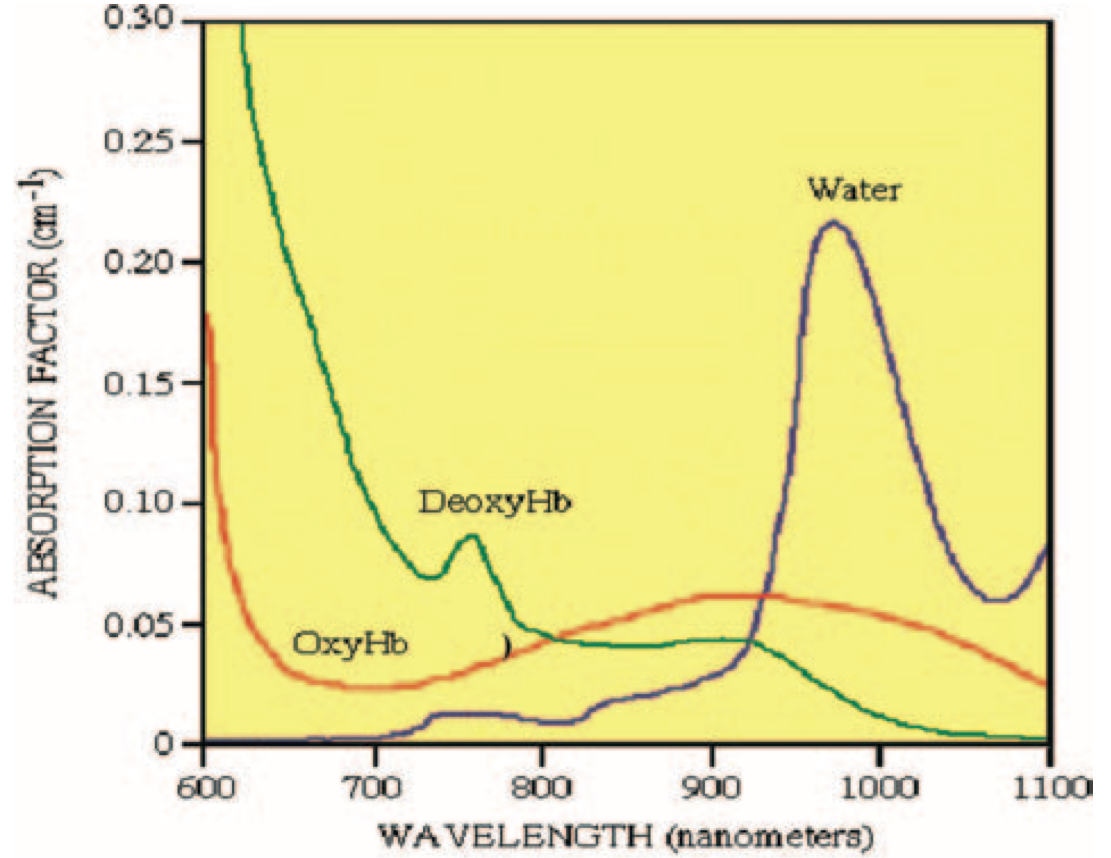
\includegraphics[width=0.8\linewidth]{AbsorptionSpectra.png}
  \end{center}
  \caption{\label{fig:fnirabsorption} Absorption spectra of water, Hb and Dhb.  From \cite{cope_1991} and \cite{horecker}}
\end{figure}
\chapter{Calculating Temperature Changes using fMRI BOLD Response}

Lorem ipsum dolor sit amet, consectetur adipiscing elit. Nullam felis justo, consequat vel semper eu, bibendum sed lectus. Fusce ultricies mi sit amet ante imperdiet eget posuere turpis volutpat. Nulla facilisi. Nulla convallis, erat et mattis bibendum, nunc velit tincidunt nisl, ac luctus massa tellus nec lectus. Pellentesque habitant morbi tristique senectus et netus et malesuada fames ac turpis egestas. Nam at venenatis sapien. In vel tortor dapibus tortor porta aliquam a sit amet diam. Nullam feugiat dignissim scelerisque. Donec rhoncus sapien eget lacus eleifend vitae adipiscing arcu mollis. Donec vel tincidunt nibh. Duis placerat scelerisque velit. Integer elementum nisl vel mi sollicitudin dictum non vel dolor. Cras consectetur consequat metus, a malesuada quam tincidunt vitae. Etiam fermentum metus nibh. Sed sollicitudin convallis faucibus. Nunc tincidunt ultricies orci, in aliquam purus interdum fermentum. \cite{sotero2011}

\section{What is BOLD}
Lorem ipsum dolor sit amet, consectetur adipiscing elit. Nullam felis justo, consequat vel semper eu, bibendum sed lectus. Fusce ultricies mi sit amet ante imperdiet eget posuere turpis volutpat. Nulla facilisi. Nulla convallis, erat et mattis bibendum, nunc velit tincidunt nisl, ac luctus massa tellus nec lectus. Pellentesque habitant morbi tristique senectus et netus et malesuada fames ac turpis egestas. Nam at \cite{galiana} venenatis sapien. In vel tortor dapibus tortor porta aliquam a sit amet diam. Nullam feugiat dignissim scelerisque. Donec rhoncus sapien eget lacus eleifend vitae adipiscing arcu mollis. Donec vel tincidunt nibh. Duis placerat scelerisque velit. Integer elementum nisl vel mi sollicitudin dictum non vel dolor. Cras consectetur consequat metus, a malesuada quam tincidunt vitae. Etiam fermentum metus nibh. Sed sollicitudin convallis faucibus. Nunc tincidunt ultricies orci, in aliquam purus interdum fermentum. 

\section{What does BOLD have to do with Temperature?}
Lorem ipsum dolor sit amet, consectetur adipiscing elit. Nullam felis justo, consequat vel semper eu, bibendum sed lectus. Fusce ultricies mi sit amet ante imperdiet eget posuere turpis volutpat. Nulla facilisi. Nulla convallis, erat et mattis bibendum, nunc velit tincidunt nisl, ac luctus massa tellus nec lectus. Pellentesque habitant morbi tristique senectus et netus et malesuada fames ac turpis egestas. Nam at venenatis sapien. In vel tortor dapibus tortor porta aliquam a sit amet diam. Nullam feugiat dignissim scelerisque. Donec rhoncus sapien eget lacus eleifend vitae adipiscing arcu mollis. Donec vel tincidunt nibh. Duis placerat scelerisque velit. Integer elementum nisl vel mi sollicitudin dictum non vel dolor. Cras consectetur consequat metus, a malesuada quam tincidunt vitae. Etiam fermentum metus nibh. Sed sollicitudin convallis faucibus. Nunc tincidunt ultricies orci, in aliquam purus interdum fermentum. 
\chapter{Conclusion}

It has been shown that by considering the entire head within the model, brain temperature can be reliably calculated from non-invasive fMRI measurements. Experimental measurements of activity-induced brain temperature changes have shown that a simple relationship does not exist~\citep{mcelligott,kiyatkin,zeschke,george,tachibana}. Single-voxel brain temperature modeling efforts predict that an increase in brain activity will induce a decrease in temperature. This one-dimensional perspective does not account for the spatial distribution of heat throughout the head like a multi-voxel approach.

Our model of brain temperature changes is able to account for the variability found in experimental brain temperature measurements.  This is accomplished by modeling heat dynamics throughout the entire head rather than reducing the model to one ROI.  It was found that the variability in experiment measurements is most likely due to differences in resting state temperatures throughout the brain.  Since each voxel is at a slightly different temperature, the same change in the BOLD response may result in different changes in temperature. Additionally, it was found through the model that a thin (4--6 mm) region of outer cortical tissue is at a resting temperature below the blood temperature.  In this region, an increase in brain activity (inducing an increase in CBF) will warm the tissue.  Thus, with the same BOLD response, tissue may either be warmed or cooled depending on it's proximity to the surface of the head.

The biggest shortcoming of our model is that we are unable to independently compare our calculations with experimental measurements of temperature and BOLD response. It was not possible for us to do this because there is currently not a method for non-invasively measuring temperature independent of an fMRI. An improvement to the model could also be gained by a more accurate method of CMRO$_2$ and CBF calculations from the BOLD response. The current method uses empirically fit formulas, so the accuracy is limited by the data used for the fitting. A model that does not rely on experimental data would be ideal. The calculations could also be improved by segmenting the head into more tissue types.  We used six tissue types, but the use of more would further improve the calculations since each tissue type has different physiological parameters (thermal conduction, baseline heat production, etc.). A separate line of research that could be pursued would be a model for calculating brain temperature changes from fNIRS data. Both fNIRS and fMRI BOLD response detect changes in local tissue oxygenation, so it should be possible to adapt our model to use fNIRS data. If such a model existed, calculations from it and our model could be compared to refine both models.

Although it is expected that the contribution would be negligible~\citep{nadel1971}, our model does not take into account the effects of perspiration. It would likely not affect the change in temperature greatly because it takes place a couple of centimeters away from brain tissue.  Another physiological affect not account for is temperature regulation by the pre-optic nucleus of the anterior hypothalamus~\citep{bertolizio2011}. It is responsible for balancing heat production and dissipation~\citep{simon1993} and if the model were applied to cases where extreme brain temperatures are created then it would be important to account for how this would react.

How human brain temperature is affected by changes in local brain activity is not well understood because the changes are small and current experimental measurement techniques may require invasive procedures. Models such as the one proposed here allow for brain temperature to be understood through non-invasive measurements such as the fMRI BOLD response.


% Bibliography
\bibliographystyle{plain}
\addcontentsline{toc}{chapter}{References}
\bibliography{thesis}
\appendix
\appendix
\addappheadtotoc
\chapter{Code}
\label{apdx:code}
The following sections include the code used.  It was written for Matlab R2011b and requires SPM8 to run.  Additionally, it is recommended that you have at least 4 GB of RAM in order to work with the large datasets that are produced.  For information about how to visualize the data produced, see~\cref{apdx:visualize}.  All of the code is available through the temptools github page (\url{https://github.com/greggroth/temptools}).  Additionally, many of the tasks can be completed using the temptools gui (\cref{fig:ttmain,fig:ttcalcequil,fig:tttempcalc,fig:ttvisualize}) which can be invoked by running
\begin{lstlisting}[style=snippet]
  temptools
\end{lstlisting}
at the Matlab command prompt (make sure the temptools directory and subdirectories have been added to the Matlab path).  The procedure used is explained in~\cref{sec:approach} and a graphical representation is available in~\cref{fig:procedureflowchart}.
\begin{figure}[bt]
  \centering
    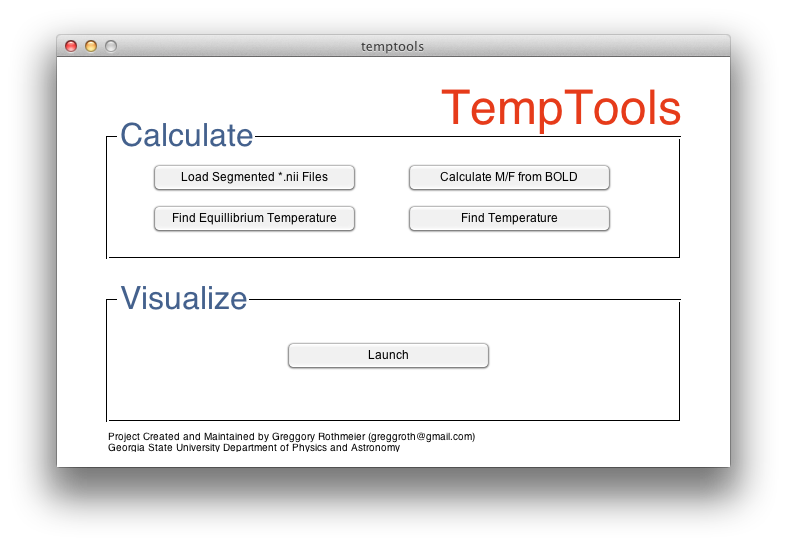
\includegraphics[keepaspectratio=true, width=17cm]{temptools/main.png}
    \caption[temptools: main window]{\label{fig:ttmain} The main window of temptools.  From here, you can go through the calculation steps and launch the visualization tool.}
  \centering
\end{figure}
\begin{figure}[bt]
  \centering
    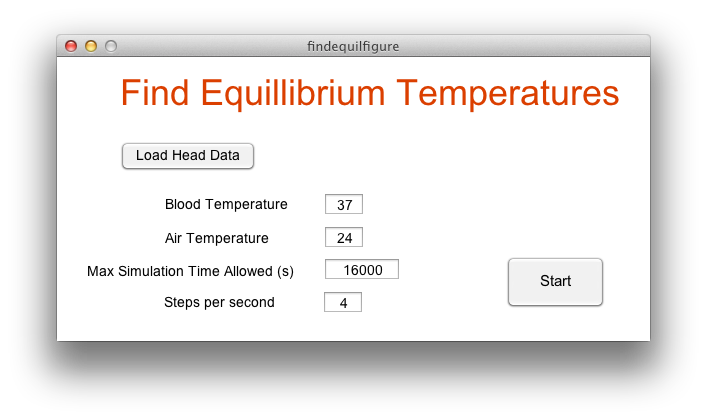
\includegraphics[keepaspectratio=true, width=17cm]{temptools/calcequil}
    \caption[temptools: calculate the equilibrium temperature window]{\label{fig:ttcalcequil} This is the interface for calculating the equilibrium temperature (method explained in~\cref{apdx:findequil}) under certain conditions.}
  \centering
\end{figure}
\begin{figure}[bt]
  \centering
    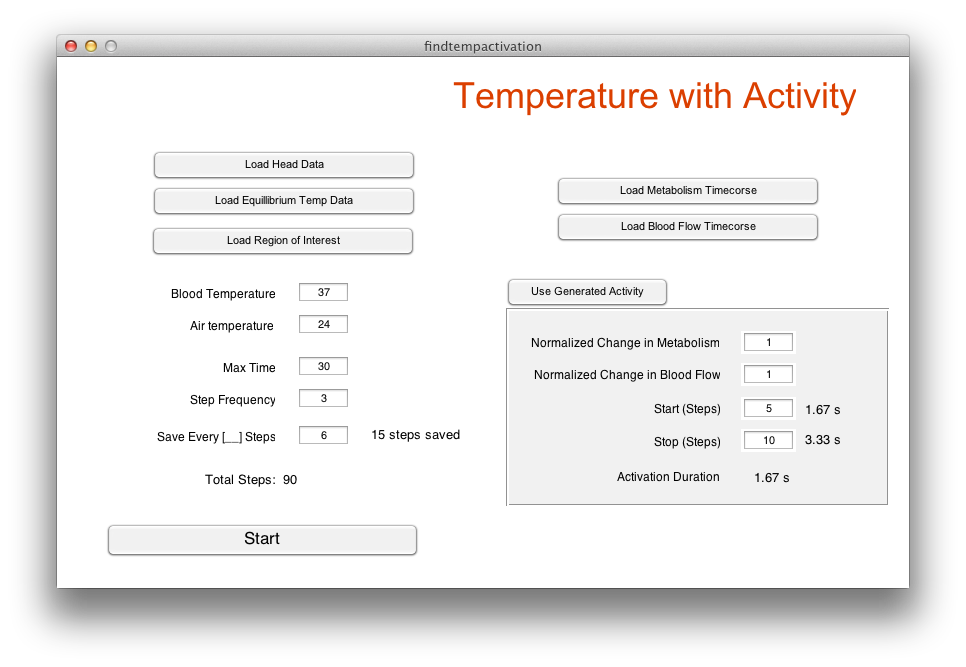
\includegraphics[keepaspectratio=true, width=17cm]{temptools/tempcalc}
    \caption[temptools: calculate temperature during activity]{\label{fig:tttempcalc} The interface for calculating temperature changes when blood flow and metabolism are time dependent.  This can be achieved by either loading metabolism and blood flow datasets or by using generated activity.}
  \centering
\end{figure}
\begin{figure}[bt]
  \centering
    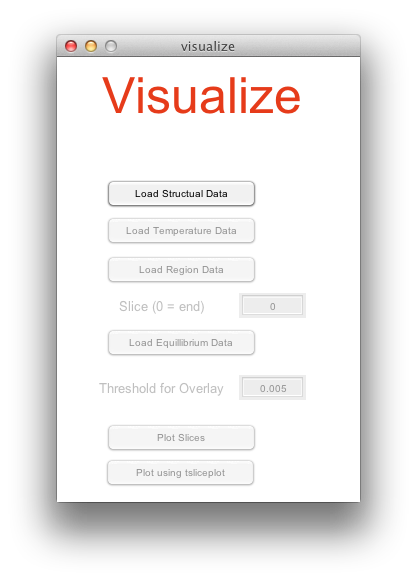
\includegraphics[keepaspectratio=true, width=10cm]{temptools/visualize}
    \caption[temptools: visualize the data]{\label{fig:ttvisualize} Visualize your data using the temptools visualization window.  This loads all of the required data and launches a slice browser or tsliceplot (see \cref{apdx:visualize} for more details).}
  \centering
\end{figure}
% Load T1/create head data
\section{Creating the Head Matrix}
\label{apdx:headmatrix}
Before any calculations can be done, a matrix containing tissue-specific parameters must be created.  First, a T1 contrast image should be segmented using SPM8 (\url{http://www.fil.ion.ucl.ac.uk/spm/software/spm8/}).  For ease of consistency, the one provided by SPM8 in ./canonical/ is best to use.  Using SPM's ``New Segmentation'' algorithim will segment the image into five different tissue types (gray matter, white matter, cerebral spinal fluid, soft tissue and bone).  Once this is complete, run ImportSegmentedT1() within this directory and it will return a matrix that has been populated with the tissue-specific parameters required for accurate temperature calculations. The functions fillAir() (\ref{code:fillair}), fillHoles() (\ref{code:fillHoles}), build\_skin() (\ref{code:buildskin}) and repair\_headdata() (\ref{code:repairheaddata}) are functions required by BulkImportNII().  More information about this procedure is in~\cref{sec:prephead}.
\subsection{ImportSegmentedT1()}
\lstinputlisting[style=codeblock]{code/ImportSegmentedT1.m}
\subsection{fillAir()}
\label{code:fillair}
\lstinputlisting[style=codeblock]{code/fillAir.m}
\subsection{fillHoles()}
\label{code:fillHoles}
\lstinputlisting[style=codeblock]{code/fillHoles.m}
\subsection{build\_skin()}
\label{code:buildskin}
\lstinputlisting[style=codeblock]{"code/build_skin.m"}
\subsection{repair\_headdata()}
\label{code:repairheaddata}
This function will go through the dataset and make sure the tissue-specific parameters are correct for the tissue type assigned for that voxel.  fillAir(), fillHoles() and build\_skin() all correct mislabeled voxels, but they only correct the tissue assignment.  After using any of these functions, the data must be passed through repair\_headdata to update the stored parameters.
\lstinputlisting[style=codeblock]{"code/repair_headdata.m"}
% Load fMRI Data
\clearpage
\section{Loading the fMRI Data}
\label{apdx:fmriprocessing}
The following sections details the processing required to convert the BOLD data (in NIFTI format) to metabolism and blood flow time-courses that can then be used to calculate temperature.
\subsection{sample\_bold\_import()}
The following code automates the procedure of processing and doing all the calculations on the dataset reported in~\citet{dhamala}.  It's is written for my data on my machine, but it can be used to gain a better understanding of the procedure. For a conceptual explanation, see~\cref{sec:calcmf}.
\lstinputlisting[style=codeblock]{"code/sample_bold_import.m"}
\subsection{avg\_NII\_rest()}
\lstinputlisting[style=codeblock]{"code/avg_NII_rest.m"}
\subsection{avg\_NII\_normalize()}
\lstinputlisting[style=codeblock]{"code/avg_NII_normalize.m"}
\subsection{BOLDtoMF()}
\lstinputlisting[style=codeblock]{"code/BOLDtoMF.m"}
\subsection{lambw() and lambw\_mex()}
The lambw() function is a wrapper for the wapr() function available on Matlab FileExchange (\url{http://www.mathworks.com/matlabcentral/fileexchange/3644-real-values-of-the-lambert-w-function/content/Lambert/wapr.m}).  A compiled version of this function (lambw\_mex()) runs much faster and is recommended.  This function is used over Matlab's built-in Lambert-W function for the sake of performance.
\lstinputlisting[style=codeblock]{"code/lambw.m"}
% Find Equilibrium
\clearpage
\section{Calculating the Equilibrium Temperature}
\label{apdx:findequil}
In order to determine the temperature fluctuations due to changes in activity, the baseline temperature must first be established for each voxel.  The function tempCalcEquilibrium() will update the temperature using the Penne's bioheat equation (\cref{eq:3dbioheat}) until the change in temperature for each voxel falls below a certain threshold.  Details about this procedure are available in~\cref{sec:calcequilT}.
\subsection{tempCalcEquilibrium()}
\lstinputlisting[style=codeblock]{code/tempCalcEquilibrium.m}
% Find Temperature Change
\clearpage
\section{Calculating the Temperature Change}
The following function takes as inputs the head data matrix (\cref{apdx:headmatrix}), the metabolism and blood flow time courses (\cref{apdx:fmriprocessing}) and the equilibrium temperatures (\cref{apdx:findequil}) and calculates the temperature time-course.   More details about this algorithm can be found in~\cref{sec:calcT}.
\subsection{tempCalcDynMF}
\label{apdx:tempCalcDynMF}
\lstinputlisting[style=codeblock]{code/tempCalcDynMF.m}
\chapter{Visualization Tools}
\label{apdx:visualize}
The temperature data is a four dimensional dataset (time, x, y and z), so good visualizations tools are necessary to analyzing the results.  The primary tool I use is a modification of SliceBrowser (\url{http://www.mathworks.com/matlabcentral/fileexchange/20604}) and is provided as part of temptools (\url{https://github.com/greggroth/temptools/tree/master/lib/SliceBrowser}).  In working with this, I also created a function (TempPlot()) to act as a wrapper and handle possible plotting situations depending on the number of inputs.
\setcounter{section}{1}
\setcounter{subsection}{0}
\subsection{TempPlot()}
\lstinputlisting[style=codeblock]{code/TempPlot.m}
\subsection{tsliceplot}
This is a visualization tool I wrote that allows you to view the change in temperature versus time for a line passing through the head.  Screenshots of the tool can be seen in~\cref{fig:tsliceplot,fig:tsliceplotz}.

Usage:
\begin{lstlisting}[style=snippet,label=invoke-tsliceplot]
  tsliceplot(temperature_data, equilibrium_temperature_data)
\end{lstlisting}

The script is available as part of temptools (\url{https://github.com/greggroth/temptools/tree/master/lib/tsliceplot}).

\begin{figure}[hbt]
  \centering
    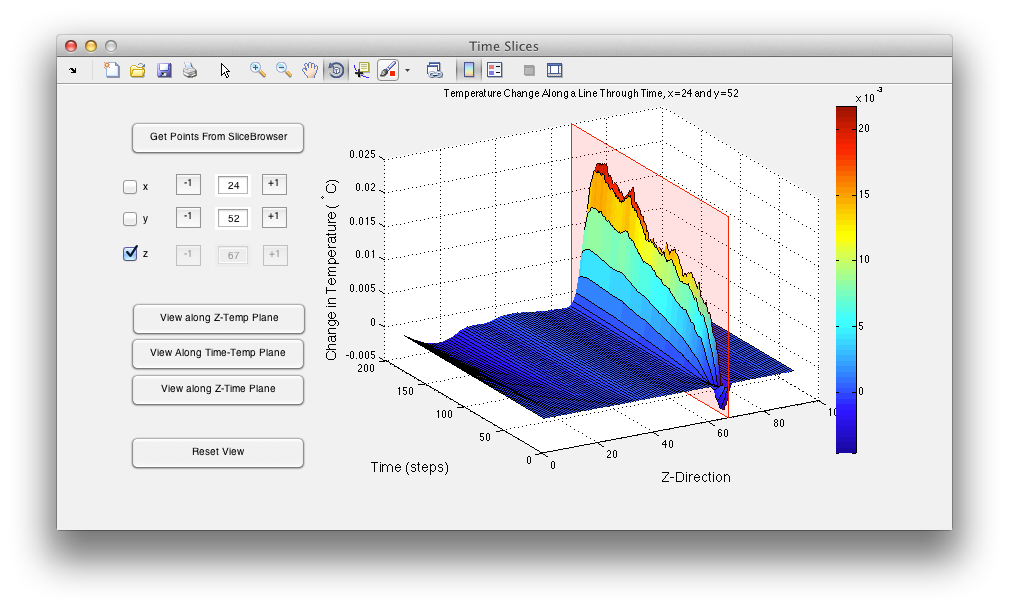
\includegraphics{tsliceplot/default-view}
    \caption[Visualization using tsliceplot]{Experimental data for activity in the motor cortex visualized with tsliceplot. \label{fig:tsliceplot}}
  \centering
\end{figure}

\begin{figure}[hbt]
  \centering
    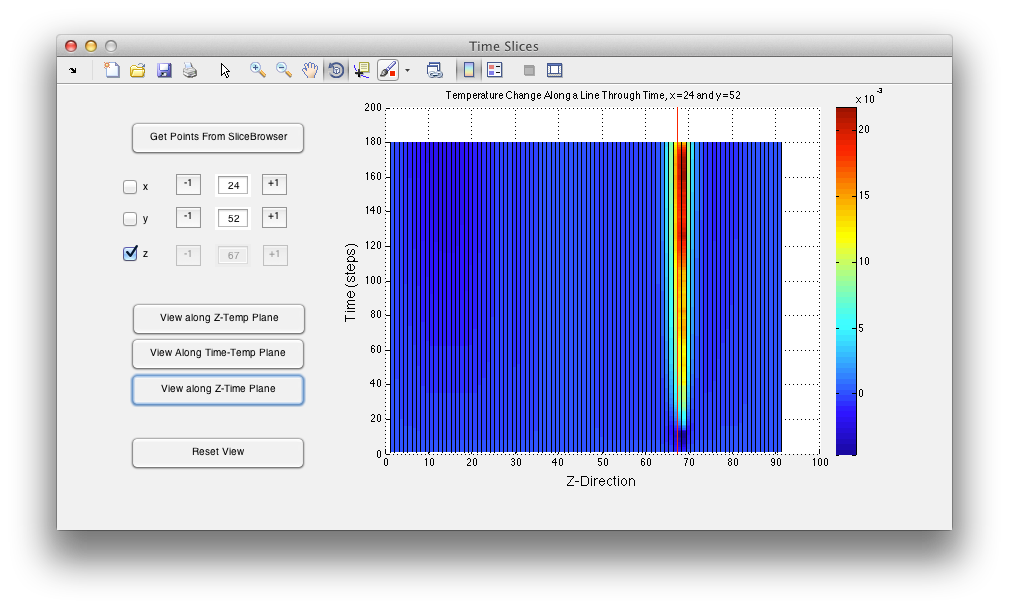
\includegraphics{tsliceplot/z-plane-view}
    \caption[Visualization using tsliceplot (z v. t plane)]{The same data as is presented in~\cref{fig:tsliceplot}, but viewed flat-on along the z vs. time plane.\label{fig:tsliceplotz}}
  \centering
\end{figure}
  
\end{document}